\documentclass[border=1mm]{standalone}

\usepackage{amsmath}
\usepackage{xcolor}
\definecolor{den-6}{HTML}{666666}
\usepackage{tkz-tab}
\usetikzlibrary{arrows}

\begin{document}

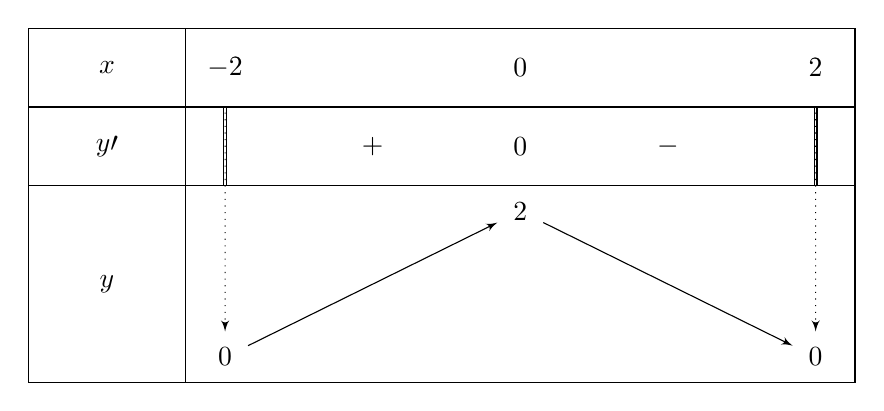
\begin{tikzpicture}
    \tkzTabInit[
        lgt=2, 
        deltacl=.5, 
        espcl=3.75]
        {$x$ / 1, $y\prime$ / 1, $y$ / 2.5}
        {$-2$, $0$, $2$}%
    \tkzTabLine{ d, +, 0, -, d}
    \tkzTabVar{-/ $0$ /, +/ $2$ /, -/ $0$}
    \tkzTabVal[draw]{1}{2}{0}{$-2$}{$0$}
    \tkzTabVal[draw]{2}{3}{1}{$2$}{$0$}
    \end{tikzpicture}

\end{document}
